\chapter{Build Your own ExG (2A)}

Now that we know how to build an opamp circuit to amplify a signal, we can build our own Electromyography or Electrocardiography circuit.  You probably noticed how sensitive the opamp circuits were to the resistor values, so we will use a specialized device called an instrumentation amplifier, which is designed to amplify weak signals by combining non-inverting amplifiers with precision matched resistances referenced to each other through a gain resistor (which controls the gain of both) that feeds into a differential amplifier setup (like an inverting amplifier of one signal with respect to a voltage divided version of the second).

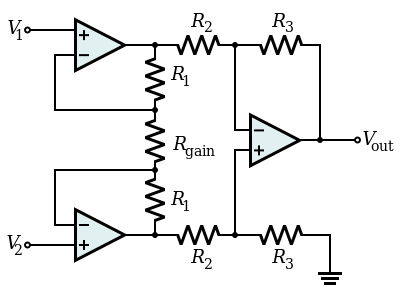
\includegraphics[width=0.4\textwidth]{../images/400px-Op-Amp_Instrumentation_Amplifier.png}

